\documentclass[aps,prb,twocolumn,superscriptaddress,floatfix]{revtex4-2}
% \usepackage[backend=bibtex]{biblatex}
% \addbibresource{B.bib}
\usepackage{amsmath,amssymb} % math symbols
\usepackage{bm} % bold math font
\usepackage{graphicx} % for figures
% \usepackage{comment} % allows block comments
% \usepackage{ulem} % allows strikeout text, e.g. \sout{text}
\usepackage{adjustbox}
\usepackage{enumitem}
\setlist{noitemsep,leftmargin=*,topsep=0pt,parsep=0pt}

\usepackage{xcolor} % \textcolor{red}{text} will be red for notes
\definecolor{lightgray}{gray}{0.6}
\definecolor{medgray}{gray}{0.4}

\usepackage{hyperref} 
\hypersetup{
colorlinks=true,
urlcolor = black,
citecolor= black,
linkcolor= blue,
% bookmarks=true,
% bookmarksopen=false,
}
\graphicspath{{Images/}}

%\date{2nd Nov 2021}
\newif\ifptitle
\newif\ifpnumber
\newcounter{para}
\newcommand\ptitle[1]{\par\refstepcounter{para}
{\ifpnumber{\noindent\textcolor{lightgray}{\textbf{\thepara}}\indent}\fi}
{\ifptitle{\textbf{[{#1}]}}\fi}}
\ptitletrue  % comment this line to hide paragraph titles
\pnumbertrue  % comment this line to hide paragraph numbers

% Allows rewriting the same title in the supplement
\newcommand{\mytitle}{ABC to Machine Learning}

\begin{document}

\title{\mytitle}

\author{Supervisor: Dr. Gareth Conduit}
\affiliation{Department of Physics, Cambridge University, Cavendish Laboratory, 19 JJ Thomson Ave, Cambridge CB3 0HE}

\newpage

\begin{abstract}

\noindent
This literature review introduces popular supervised machine learning methods from regression to the physics-informed neural network and their perspective strength and limitations. Then two case studies of applications of machine learning in various fields of physics research such as material science and astronomy are discussed. 
\end{abstract}

\maketitle

\section{Introduction}
Machine learning is an intriguing field of study that empowers computer systems to learn from data without being explicitly programmed. Its applications encompass various functions such as prediction, classification, and pattern detection\cite{towardsdatascienceMachineLearning}. Machine learning can be subdivided into three categories: supervised, unsupervised, and reinforcement learning. This review will primarily focus on supervised learning, as it is the most prevalent machine learning technique within research for making predictions. Some of the most commonly seen supervised machine learning methods include regression, neural work/deep neural network, decision tree, gaussian process, and physics-informed neural network. Their strengths and limitations, along with their applications will be discussed in this review.
\section{Supervised learning}
Supervised learning is a machine learning technique that uses labeled data to train a model to make predictions. The model is trained by comparing the predicted output with the true output and then adjusting the parameters of the model to minimize the error. The model is then tested on a test set to evaluate its performance\cite{ibmWhatSupervised}.
Supervised learning breaks down into two different types of problems: regression and classification.
Regression is the task of predicting a continuous value, such as a certain physical property of a material, while classification is the task of predicting a discrete value, such as the classification of astronomical objects into galaxies and stars.
Due to the nature of their output, regression and classification have different methods of evaluation. For regression, the most common evaluation metric is the mean squared error (MSE), which is the average of the squared difference between the predicted value and the true value. For classification, the most common evaluation metric is accuracy, which is the fraction of the data points that are correctly classified.

\section{Supervised Machine learning methods}
There is a list of various machine learning methods. In this section, we will discuss some of the most common machine learning techniques used in research, including regression, neural network, decision tree, gaussian process and finally, physics-informed machine learning.

\subsection{Regression Methods}
Although the idea of machine learning was first introduced in 1959
\cite{samuel1959some},
the most fundamental technique involved in machine learning dates way back to the 18th century when the first curve-fitting technique was introduced. Curve fitting is a process of construction a mathematics function, that has the best fit to a series of data points. It remains one of the most theoretically challenging parts of machine learning\cite{towardsdatascienceDeepDive}.\\
\paragraph{Linear regression}
The most basic and commonly seen fitting technique is a first-order polynomial equation, also known as linear regression:
\begin{equation}
    y=ax+b
\end{equation}
which is a straight line that connects two points with distinct x coordinates.\\

\paragraph{Polynomial Regression and Taylor Theorem}
With more than two data points to fit,  we could always add a term of higher power of $x$, to make it a quadratic equation
\begin{equation}
    y= ax^2 +bx+ c
\end{equation}
or another term to construct a cubic regression:
\begin{equation}
    y= ax^3 +bx^2 + cx+d
\end{equation}
In general, many data are not related by a simple linear relationship, we can construct a polynomial regression of any order, by adding more terms to the equation.
This method is identical to Taylor expansion around a certain point 
$$f(x)=\sum_{n=0}^{\infty} a_n(x-b)^n$$
The find the value of the parameters, we mini
mize the ordinary least squares:
\begin{equation}
    \sum{y_i-(kx_i+c)}^2
\end{equation}

The limitation of Taylor expansion comes when the $x$ becomes infinitely large, which will cause the magnitude of $y$ to become infinitely large, which may not reflect the datasets properly. \\

\paragraph{Padé approximant}
As a further improvement to Taylor expansion, Padé approximant was developed by Henri Padé around the year 1890 to fit curves using the ratio of two polynomials\cite{wikipediaPadApproximant}.
An $[N/M]$ Pade approximant is formed of a $N$th-degree polynomial on the numerator and an $M$th-degree polynomial on the denominator:
\begin{equation}
    P(x)=\frac{a_0+a_1 x+a_2x^2+... a_Nx^N}{b_0+b_1 x+b_2x^2+... b_Mx^M}
\end{equation}
\cite{wolframPadApproximant}
Padé approximant $\frac{ax^2+bx^3+...}{c+dx+...+x^6}$ making sure that $f(x)$ does not tend to infinity at large x, in this case, tend to $1/x$.\\
Padé approximant is superior to the Taylor series when describing a function that contains poles. Also, by dividing a polynomial by another, the Pade approximant prevents the function from diverging by letting $N<=M$. However, the Padé approximant is limited to low dimensional data and little noise\cite{deringer2021gaussian}. 
Pade Approximant inspired the development of neural network\cite{TaylorSeries}, a systematic method to introduce non-linearity into the curve-fitting model, which also is the next topic we will discuss.\\

\subsection{Neural network}
In the previous cases, we discussed regression techniques for a single variable function, while in physics, a function is usually higher dimensional. The limitation comes in when the number of independent variables becomes more than 1. For example, $y$ is now a function of $x_1$ and $x_2$. i.e. $y(x_1,x_2)$.
In this case, we would have to include a term such as $x_1x_2$ and $x_1x_2$, which means that the number of coefficients we used now grows exponentially to the number of independent variables. This is where the neural network comes in and solves the problem. A neural network consists of a series of nodes, each with its own weight and bias, and the results are fed into a non-linear activation function, such as a sigmoid function, to produce the output.
A model is built with one layer of nodes and its weights and bias is usually randomly assigned or set to zero.
After assigning weights and biases in the model, the next step is to reduce the loss function in the neural network. Back-propagation is a way of propagating the total loss back into the neural network to know how much of the loss every node is responsible for, and subsequently updating the weights in a way that minimizes the loss by giving the nodes with higher error rates lower weights, and vice versa. This process is repeated until the loss function is minimized

\paragraph{Deep Neural Network}
Neural networks (NN) have a large number of tunable parameters, all of which fall into two categories\cite{George_2018}. The first type is internal parameters, weights $w_i$ and bias $b$. The weights and biases are selected via an optimization routine (e.g., gradient descent) over a chosen metric (e.g., mean squared error). These two parameters are discussed in the previous section.
The hyperparameters include width, which is the number of nodes per layer, and depth, which is the number of layers stacked to form the network. The depth and width of neural networks are usually pre-set by developers, though a few combinations can be tried to obtain the best model. A deeper and wider neural network generally has a better performance than a shadower and narrower neural network, however, it is also more expensive to train.
\cite{Hinners_2018}
\begin{figure}[h]
    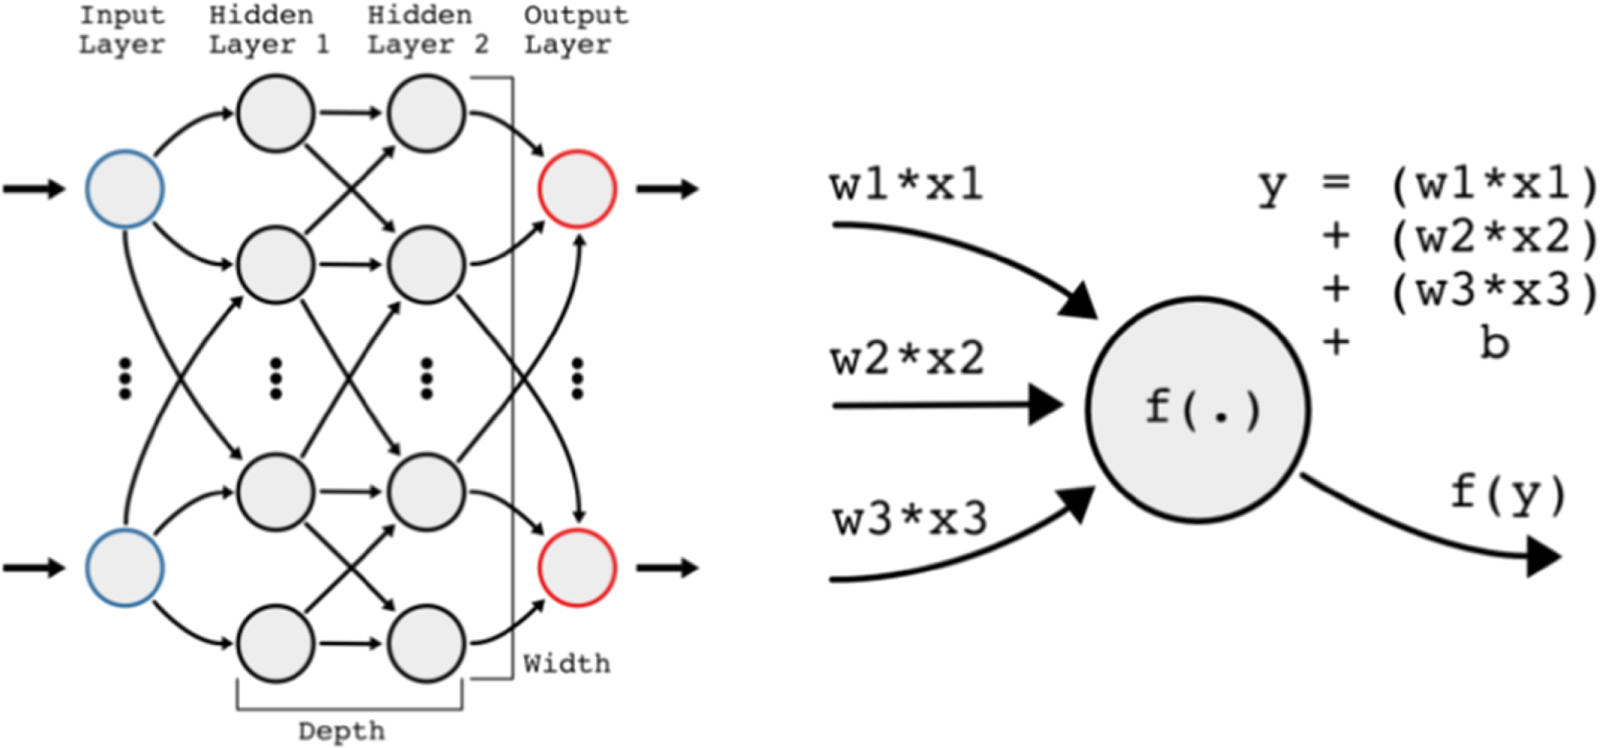
\includegraphics[clip=true,width=\columnwidth]{NN.jpeg}
    \caption{Left: Schematic for a simple artificial neural network with a depth of two and unspecified width. Right: Schematic for a simple, generic node. Here three inputs $x_i$ are scaled by weights $w_i$, summed, and biased b before being fed through an activation function $f(y)$\cite{Hinners_2018}.}
\end{figure}
In a deep neural network, each node takes some number of inputs $x_i$, combines them, feeds them through an activation function, and the result is then passed on to some other nodes in the next layer. The combination of inputs is usually multiplied by an individual weight,$w_i$, then added along with a bias term,$b$. 
The activation function is a predetermined function, such as ReLU Function, Binary Step Function, and hyperbolic tangent function. It takes in a real value and spits out a value between (0 to 1) to add non-linearity to the network\cite{v7labsActivationFunctions}.
The limitation of neural networks includes their requirement for a very large amount of data to demonstrate significantly better performance compared to other techniques. It is also extremely expensive to train due to complex data models.
Another limitation of the neural network is that the model itself is a black box and it is hard to interpret the model.
\subsection{Decision Trees}
Apart from the most commonly seen neural network, there are a few other methods that are more compatible under certain circumstances. One of them is a decision tree.
A decision tree is a popular method for classification problems in supervised machine learning. The decision tree model predicts a value of a target variable, usually categorical, based on input variables.
\cite{Rokach2014DataMW}
The decision tree is presented as a tree-like structure, where each internal node represents a test on an attribute, each branch represents the test outcome, and each leaf node represents a class label.
\begin{figure}[h]
    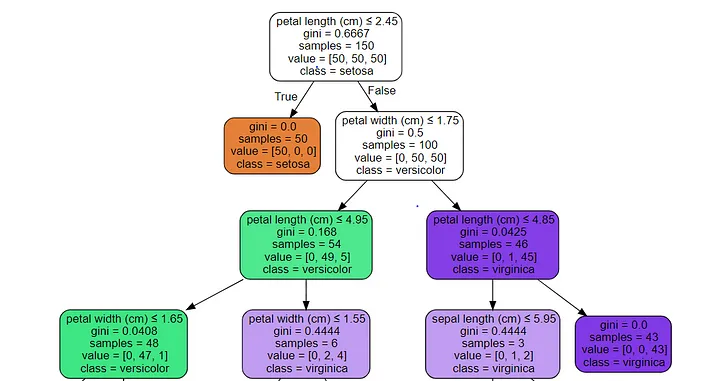
\includegraphics[clip=true,width=\columnwidth]{DT.png}
    \caption{Example of a Decision Tree model on the categorization of iris}
\end{figure}
At each node, the tree is split into branches based on the value of the attribute. The tree is built recursively until the stopping criteria are met. The stopping criteria can be the maximum depth of the tree, and the minimum number of samples in a leaf node.
At each node, the algorithm selected the correct attributes by lowering the Gini score or reducing entropy.
\cite{shalev2014understanding}
The fundamental benefit of the decision tree lies in its easy-to-understand and interpretable nature. Furthermore, it has a minimum data requirement: the data do not require cleaning or normalization before being fed to the model.\cite{quinlan1986induction}
Significant drawbacks of the decision tree method include its inaccuracy in extrapolating data and its limitation in predicting continuous values\cite{ibmWhatDecision}
\cite{scikitlearn110Decision}.

\subsection{Gaussian Process}
Gaussian Process is a non-parametric method that can be used for regression and classification problems. The function is assumed to be drawn from a Gaussian process, which is a collection of random variables, any finite number of which have a joint Gaussian distribution. The Gaussian process is defined by a mean function and a covariance function. The mean function is a function that describes the average value of the function $f(x)$, and the covariance function is a function that describes the covariance between two points $x_1$ and $x_2$\cite{perger2021auto}\cite{RePEc:eee:transb:v:146:y:2021:i:c:p:88-110}.

The distinctive feature of the Gaussian process is that it provides a probabilistic interpretation of the model instead of a point of estimation in other methods. This probabilistic representation allows for the quantification of uncertainty in the predictions, making GPs particularly useful in cases where uncertainty needs to be taken into account.

Another strength of the Gaussian Process is that it works with small sets of data very well, making them particularly useful in cases where data is limited or expensive to collect.

Examples of GPR implementation can be found in the Scikit-learn library for Python\cite{pedregosa2011scikit}.
\subsection{Physics informed machine-learning}
The method introduced in the previous section works independently of any physical formula. However, in many situations, we know partially the physical constraints in our system. These constraints can be integrated into our model to improve performance. Physics-informed neural network (PINN) is a fast-growing field in machine learning. Usually, based on the amount of available data and knowledge in physics, we can subcategorize a machine-learning problem into three cases.
\begin{enumerate}
    \item In the case of a well-developed understanding of the physical laws behind the system, i.e. the governing partial equations, initial condition, and boundary condition, we do not require a data-intensive approach to have a good understanding of the system.
    \item On the contrary, in the case of little knowledge of the physical law, we can use a general machine learning method to find patterns and insights from the data, provided that a big set of experimental data is available.
    \item In the last case, we have some physics and some data, probably missing some data or values for parameters in the partial differential equations. We can use neural networks that are specifically made to respect the physical laws, and PINN is best suited to solve this problem.
    \cite{2019JCoPh.378..686R}
\end{enumerate}
Introducing a physics-informed neural network (PINN) with observational, inductive or learning biases will allow the model to learn bearing the physics constraints of the problem\cite{benmoseleyWhatPhysicsinformed}
\cite{karniadakis2021physics}.
Physics-informed neural network (PINN) is an ML model designed to embed the PDEs into the loss function of a neural network using automatic differentiation. We will use viscous Burgers' equations as an example:
$$
\frac{\partial u}{\partial t}+u \frac{\partial u}{\partial x}=v \frac{\partial^2 u}{\partial x^2}
$$
with a suitable initial condition and Dirichlet boundary conditions. In the figure, the left (physics-uninformed) network represents the surrogate of the PDE solution $u(x, t)$, while the right (physics-informed) network describes the PDE residual $\frac{\partial u}{\partial t}+u \frac{\partial u}{\partial x}-v \frac{\partial^2 u}{\partial x^2}$. 
The loss function includes a supervised loss of data measurements of $u$ from the initial and boundary conditions and an unsupervised loss of PDE:
$$
\mathcal{L}=w_{\text {data }} \mathcal{L}_{\text {data }}+w_{\mathrm{PDE}} \mathcal{L}_{\mathrm{PDE}}
$$
where
$$
\begin{gathered}
\mathcal{L}_{\mathrm{data}}=\frac{1}{N_{\mathrm{data}}} \sum_{i=1}^{N_{\mathrm{data}}}\left(u\left(x_i, t_i\right)-u_i\right)^2 \quad \text { and } \\
\mathcal{L}_{\mathrm{PDE}}=\left.\frac{1}{N_{\mathrm{PDE}}} \sum_{j=1}^{N_{\mathrm{PDE}}}\left(\frac{\partial u}{\partial t}+u \frac{\partial u}{\partial x}-v \frac{\partial^2 u}{\partial x^2}\right)^2\right|_{\left(x_j, t_j\right)}
\end{gathered}
$$
Here $\left\{\left(x_i, t_i\right)\right\}$ and $\left\{\left(x_j, t_j\right)\right\}$ are two sets of points sampled at the initial/boundary locations and in the entire domain, respectively, and $u_i$ are values of $u$ at $\left(x_i, t_i\right)$; $w_{\text {data }}$ and $w_{\text {PDE }}$ are the weights used to balance the interplay between the two loss term.
PINN is one of the more recent topics introduced in machine learning toolboxes. Its implementation is more complicated as there is currently no well-documented official library yet. In the future, we would expect to see more development in this method.

\section{Choosing ML techniques}
The most suitable ML model is task-specific, the factors that should be considered when choosing a model are:
\begin{enumerate}
    \item The nature of output the problem, i.e. whether it is a classification or regression problem.
    \item The amount of data and resources available for training.
    \item The interpretability and complexity of the model.
\end{enumerate}
A summary of the strength and limitations of Machine learning techniques is shown in Table 1 below.\\
\begin{table}[h]
    \begin{adjustbox}{width=\columnwidth,center}
    \begin{tabular}{|l l l l l|}
        \hline ML Method & Requirement for data & Computational resource & Interpretibility & $\begin{array}{l}\text { Other } \\
        \text { advantage/limitation }\end{array}$ \\
        \hline \hline Decision Tree & Little requirement & Relatively few & $\begin{array}{l}\text { Good with a nice } \\
        \text { visualisation (tree } \\
        \text { diagram) }\end{array}$ & $\begin{array}{l}\text { Limited capability for } \\
        \text { regression, }\end{array}$ \\
        \hline Linear Regression & Average & Relatively few & Good & $\begin{array}{l}\text { Could not handle non- } \\
        \text { linear cases. Less prone to } \\
        \text { overfitting }\end{array}$ \\
        \hline Neural Network & $\begin{array}{l}\text { Perform well with Large } \\
        \text { amount of data points }\end{array}$ & $\begin{array}{l}\text { Computationally } \\
        \text { Expensive }\end{array}$ & $\begin{array}{l}\text { Black-box, hard to } \\
        \text { interpret result }\end{array}$ & Prone to over-fitting \\
        \hline Deep Neural Network & $\begin{array}{l}\text { Perform well with Large } \\
        \text { amount of data points }\end{array}$ & $\begin{array}{l}\text { Even more } \\
        \text { Computationally } \\
        \text { Expensive }\end{array}$ & $\begin{array}{l}\text { Black-box, hard to } \\
        \text { interpret result }\end{array}$ & Prone to over-fitting \\
        \hline Gaussian Process & $\begin{array}{l}\text { Perform well with limited } \\
        \text { amount of data points }\end{array}$ & $\begin{array}{l}\text { Computationally } \\
        \text { expensive }\end{array}$ & $\begin{array}{l}\text { Black-box, hard to } \\
        \text { interpret result }\end{array}$ & Gives uncertainty estimate \\
        \hline
    \end{tabular}
    \end{adjustbox}
    \caption{Summary for the strength and limitations of machine learning techniques.}
\end{table}

It is also a common practice to use more than one model, or the same model with various hyperparameters can be used to compare the performance of the model. 
In the following section, I will give two case studies in two distinctive fields of physics research to demonstrate the application of machine learning in addressing regression and classification problems respectively.
\section{Case study 1: Using a neural network to design new material}

This case study is an example of using a neural network to solve a material design problem \cite{conduit2017design}.

In this research, a new polycrystalline nickel-base superalloy was proposed by the mode that has the optimal combination of cost, density, $\gamma'$ phase content and solvus, phase stability, fatigue life, yield stress, ultimate tensile strength, stress rupture, oxidation resistance, and tensile elongation.

The construction and validation of the model are done in the following order:
Firstly, predictive models are constructed
for each property.
Then, these models are used to calculate the probability that a proposed composition fulfills a target specification.
Finally, the model searches through the composition space for an alloy that would most likely to fulfill all the specifications.

With a proposed alloy from the model, an experiment is then carried out to test the physical properties of the new alloy. Comparisons are made between the prediction from the neural network model and experimental data. The results are shown in the figure \ref{fig:NN_results},
\begin{figure}[h]
    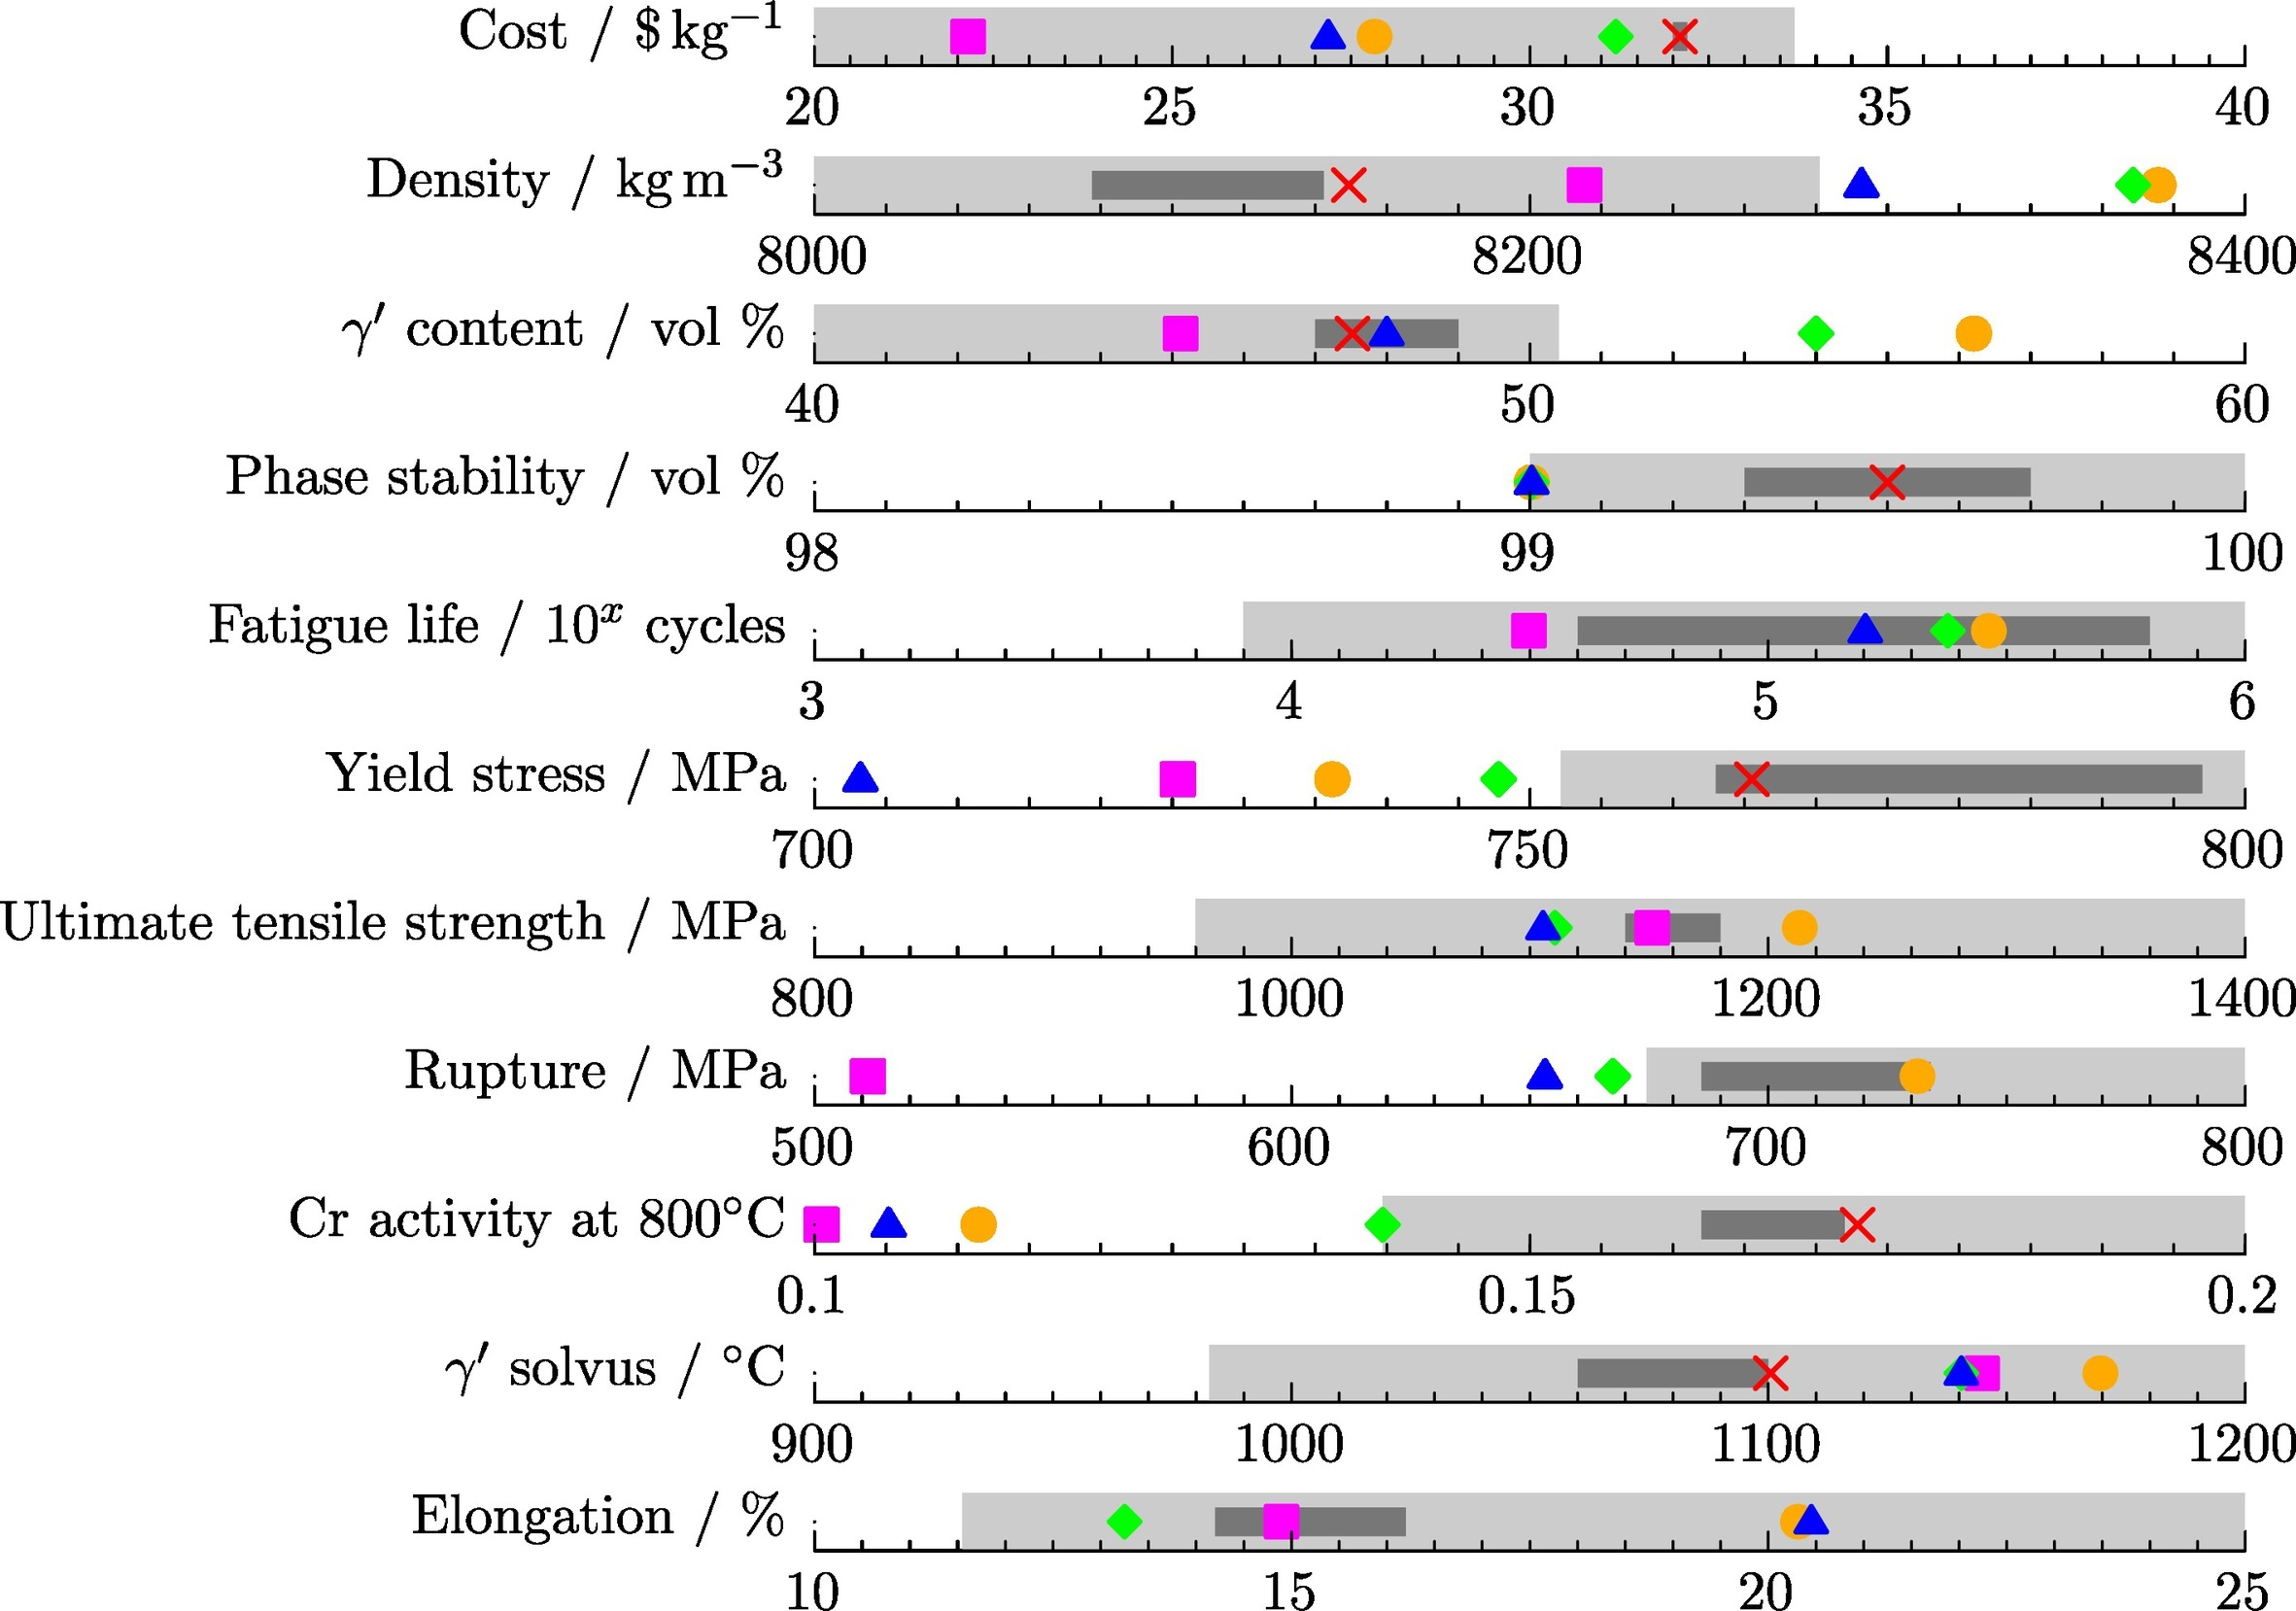
\includegraphics[clip=true,width=\columnwidth]{CS_NN_results.jpeg}
    \caption{Experimental results of the proposed alloy. For each listed property the gray box refers to the acceptable target properties, and the dark gray is the three-sigma uncertainty on the theoretical prediction. The points refer to experimentally measured values with V210A where measured}
    \label{fig:NN_results}
\end{figure}
demonstrating a successful application of machine learning in material design. The model in this case is validated by an experiment instead of cross-validation, which adds more credibility to the model
\section{Case Study 2: Machine learning in galaxy morphology classification}
This case study is chosen as it is a good example of using machine learning to replace human data labeling in classification problems in astrophysics\cite{rodirguezarticle}.
The morphological classification of galaxies provides crucial astronomical insights and helps to understand how galaxies form and evolve.
In this research, scientists classify samples into four categories: spirals, ellipticals, mergers and stars\cite{reza2021galaxy}. The researcher tested 5 various models (Decision Tree, Random Forest, Extra Trees, K-nearest Neighbours, Artificial Neural Network) using data from Sloan Digital Sky Survey and labeled data from Galaxy Zoo\cite{zooniverseZooniverse}. 
\begin{figure}[h]
    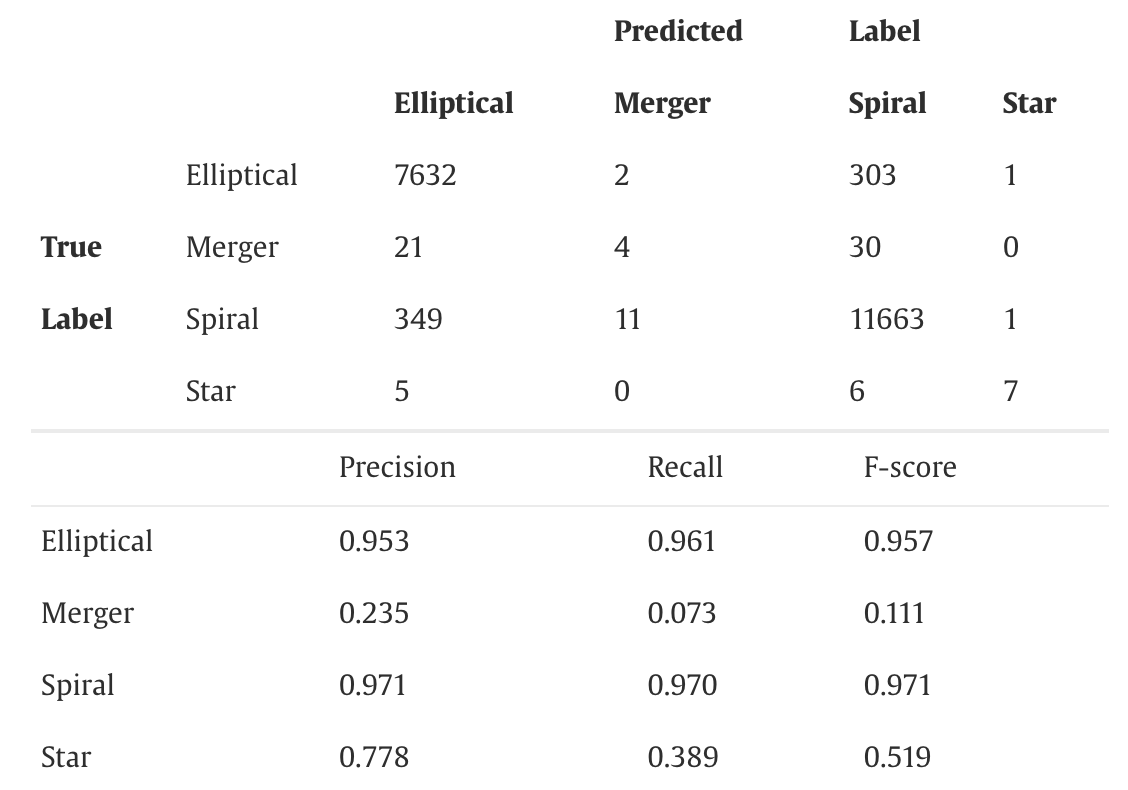
\includegraphics[clip=true,width=\columnwidth]{CS_Galaxy_DT.PNG}
    \caption{Confusion Matrix showing the performance of Decision Tree model}
    \label{fig: DT}
\end{figure}
The results from the decision tree method are shown in Figure \ref{fig: DT}. The results are summarised in a confusion matrix, which shows the performance of the model in classifying each class. The diagonal elements of the matrix show the number of correct classifications, while the off-diagonal elements show the number of misclassification. The results show that the model is relatively good at classifying spirals and ellipticals, but not for mergers and stars.
\begin{figure}[h]
    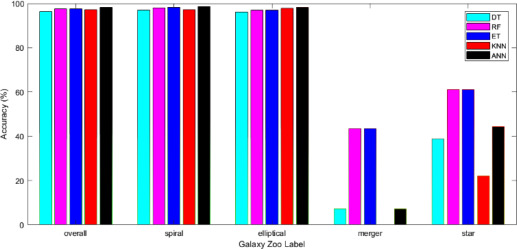
\includegraphics[clip=true,width=\columnwidth]{CS_Galaxy_Result.jpg}
    \caption{Bar chart showing overall accuracy and classwise recall using different ML algorithms}
    \label{fig: Result}
\end{figure}
The results in Figure \ref{fig: Result} shows a relatively similar performance of all five models, with all the model performing relatively well in classifying spirals and ellipticals, but not so well in classifying mergers and stars. This is a good example of a class imbalance problem in machine learning when there are many more instances of a certain class (i.e.elliptical and spiral galaxies) than other classes (i.e.mergers and stars).
This case study demonstrated that machine learning is a powerful tool for classification problems which is a rather labor-intensive task had it done by human labeling. Various methods could produce similar results, but the choice of method is task-specific. However, machine learning is far from being a perfect solution as certain problems such as class imbalance problems would need more fine-tuning or perfection of data.

\section{Conclusion}
Machine learning is a powerful tool that can be applied in physics, given a mass quantity of data we can train the model and predict the outcome of the system. One should carefully choose a model based on the amount of data points available, the complexity and the interpretability of the model. Machine learning and its black-box nature result in a lack of interpretability, as well as a good reflection of the physical property of the system. However, the performance of the model can be further improved by incorporating existing physical laws into the model, or by recognizing the relevant symmetry in the model itself. There are already attempts to integrate physical law. In the future, we may see an increasing number of physics-informed machine-learning models.

\bibliographystyle{unsrt} 
\bibliography{B.bib}
\end{document}